% \input{"IAB/latex/TeX-Folienformat.tex"}
\input{"/Users/jonathanlatner/Google Drive/My Drive/IAB/latex/TeX-Folienformat.tex"}

\documentclass[t,8pt,utfx8]{beamer}
\usepackage{booktabs}
\usepackage{setspace}
\usepackage{parskip}
\usepackage{graphicx}
\usepackage{subcaption}
\setbeamertemplate{caption}[numbered]
\newcommand{\sprache}{\englisch}
\renewcommand{\thesubsection}{\alph{subsection})}
\usepackage[cal=pxtx, scr=dutchcal]{mathalpha}


\usepackage{listings} %include R code

\definecolor{codegreen}{rgb}{0,0.6,0}
\definecolor{codegray}{rgb}{0.5,0.5,0.5}
\definecolor{codepurple}{rgb}{0.58,0,0.82}
\definecolor{backcolour}{rgb}{0.95,0.95,0.92}

\lstdefinestyle{mystyle}{
    backgroundcolor=\color{backcolour},   
    commentstyle=\color{codegreen},
    keywordstyle=\color{magenta},
    numberstyle=\tiny\color{codegray},
    stringstyle=\color{codepurple},
    basicstyle=\ttfamily\tiny,
    breakatwhitespace=false,         
    breaklines=true,                 
    captionpos=b,                    
    keepspaces=true,                 
    numbers=left,                    
    numbersep=5pt,                  
    showspaces=false,                
    showstringspaces=false,
    showtabs=false,                 
    columns=fullflexible,
    frame=single,
    tabsize=2
}

\lstset{style=mystyle}


\newcommand{\btVFill}{\vskip0pt plus 1filll}

\title{Generating synthetic data is complicated: Know your data and know your generator}
\subtitle{Wiesbaden, \newline 21. März, 2024}

\author{Jonathan Latner, PhD \newline Dr. Marcel Neuenhoeffer \newline Prof. Dr. Jörg Drechsler}

\newcounter{noauthorlines}
\setcounter{noauthorlines}{2} % Wert für 2 Autoren über 2 Zeilen. Ggf. anpassen

% %%%%%%%%%%%%%%
% Ende Anpassung
% %%%%%%%%%%%%%%

% \input{"IAB/latex/TeX-Folienformatierung_CD_2019"}
\input{"/Users/jonathanlatner/Google Drive/My Drive/IAB/latex/TeX-Folienformatierung_CD_2019"}

% Modify the section in toc template to enumerate
\setbeamertemplate{section in toc}{%
    \inserttocsectionnumber.~\inserttocsection\par
}

% use for subsections
% \setbeamertemplate{subsection in toc}{}
\setbeamertemplate{subsection in toc}{%
    \setlength{\parskip}{1mm}
        \hskip2mm -- \hskip1mm\inserttocsubsection\par
}


\usepackage{colortbl}
\definecolor{lightgray}{gray}{0.9}


\begin{document}


\frame[plain]{\titlepage}

\begin{spacing}{1.25}

\section{Introduction}\label{sec:intro}
\frame{\frametitle{}
Section \ref{sec:intro}: Introduction
}

\frame{\frametitle{What is our goal today?}

\begin{itemize}
    \item Common perception that making synthetic data is easy
    \item We want to show that its complicated
    \begin{itemize}
        \item You need to know your data
        \begin{itemize}
            \item Missing values, messy data, etc.
        \end{itemize}
        \item You need to know your generator
        \begin{itemize}
            \item How does it deal with missing values?
            \item How efficient is it (data dimensionality)?
            \item How does it meet privacy standards?
        \end{itemize}
    \end{itemize}
    \item Conclusion
    \begin{itemize}
        \item There is no one, single solution to creating synthetic data
        \item The right generator depends on the goal
        \item Eventually \dots make some recommendations (but not today)
    \end{itemize}
\end{itemize}
}

\frame{\frametitle{The good news -- making synthetic data is easy}

\begin{itemize}
    \item \url{Gretel.ai}: The synthetic data platform for developers. Generate artificial datasets with the same characteristics as real data, so you can develop and test AI models without compromising privacy.
    \item \url{Mostly.ai}: Synthetic Data. Better than real. Still struggling with real data? Use existing data for synthetic data generation. Synthetic data is more accessible, more flexible, and simply...smarter.
    \item \url{Statice.ai}: Generating synthetic data comes down to learning the joint probability distribution in an original, real dataset to generate a new dataset with the same distribution.  The more complex the real dataset, the more difficult it is to map dependencies correctly. Deep learning models such as generative adversarial networks (GAN) and variational autoencoders (VAE) are well suited for synthetic data generation.
    \item \url{hazy.com}: Synthetic data does not contain any real data points so can be shared freely. Say goodbye to lengthy governance processes associated with real data.  Specifically, Hazy data is designed to preserve all the patterns, statistical properties and correlations in the source data, so that it can be used as a drop-in replacement for it.
    \item DataSynthesizer: The distinguishing feature of DataSynthesizer is its usability — the data owner does not have to specify any parameters to start generating and sharing data safely and effectively.
\end{itemize}
}

\frame{\frametitle{The bad news -- making synthetic data is hard}

\begin{itemize}
    \item According to the Alan Turing Institute (Jordan et al., 2022)
    \item How do we evaluate utility (and fidelity)? There is no one measure of either.
    \begin{itemize}
        \item Utility and fidelity are sometimes called general/broad and specific/narrow measures within the single concept of utility (Snoke et al., 2018; Drechsler and Reiter, 2009). 
    \end{itemize}
    \item Efficiency (i.e. duration in time) is important and often ignored.  The algorithm should scale well with the dimension of the data space in a relational way, not exponential way.
    \item How do we evaluate privacy?
    \begin{itemize}
        \item Is privacy a function of the generator? 
        \item Is privacy a function of the data? 
    \end{itemize}
\end{itemize}
}



\frame{\frametitle{Our goal is to illustrate the challenges}
\begin{itemize}
    \item Know your generator
    \begin{itemize}
        \item Evaluate 3 synthetic data generators (SDG): DataSynthesizer, CTGAN, Synthpop
        \item How do they actually create data?
        \item How efficient are they with respect to data dimensionality?
        \item Thinking about what this means for privacy (not today)
    \end{itemize}
    \item Know your data (1 dataset, 2 utility measures)
    \begin{itemize}
        \item Cleaning/pre-processing
        \item Utility: Propensity score mean-squared error (pMSE) - Append the original and synthetic datasets. Creating an indicator variable for original/synthetic datasets.  For each record in the combined dataset ($n$) the probability of being in the synthetic dataset is computed via logistic regression; this is the propensity score ($p$).  Lower scores are better.  ($pMSE = \frac{1}{N}\sum_{i=1}^{N}[\hat{p}_i - c]^2$)
        \item Ratio of counts/estimates (ROC/ROE) - Calculate the ratio of each value in a given variable for both synthetic/original datasets.  Then, calculate the ratio of each value for each dataset, and divide the smaller of these two estimates by the larger one.  Higher scores are better.  ($ROE = \frac{min(y_orig^1,y_synth^1)}{max(y_orig^1,y_synth^1)}$)
    \end{itemize}
\end{itemize}
}


\section{Know your data (SD2011)}\label{sec:data}
\frame[c]{\frametitle{}
\centering
Section \ref{sec:data}: Know your data (SD2011)
}

\frame{\frametitle{Real data}
\begin{itemize}
    \item Social Diagnosis 2011 (SD2011)
    \item Loads with Synthpop
    \begin{itemize}
        \item \url{http://www.diagnoza.com/index-en.html}
        \item Not entirely clear how original data is created or cleaned to create data in Synthpop
    \end{itemize}
    \item Like real data, has `quirks' or unusual values/variables
    \begin{itemize}
        \item Includes missings
        \begin{itemize}
            \item Informative (i.e. month married, but single)
            \item Non-informative 
        \end{itemize}
        \item Includes `errors'
        \begin{itemize}
            \item \texttt{smoke} - Does not smoke is NO, but \texttt{nociga} - 20/22 cigarettes per day 
            \item \texttt{bmi} = 451, but \texttt{height} = 149 and \texttt{weight} = NA (999)
        \end{itemize}
        \item Includes generated variables (Can be problematic for SDGs)
        \begin{itemize}
            \item \texttt{bmi,agegr}
        \end{itemize}
    \end{itemize}
\end{itemize}
}


\frame{\frametitle{Data (SD2011)}
\vskip -5mm
\begin{table}[ht]
    \centering
    \vskip -2mm
    \rowcolors{1}{white}{lightgray}
    \resizebox{\textwidth}{!}{% latex table generated in R 4.4.0 by xtable 1.8-4 package
% Thu Sep 26 09:11:53 2024
\begin{tabular}{rlllllllll}
  \toprule
Number & Variable & Description & Type & Observations & Unique.Values & Missings & Negative.values & Generated & Messy \\ 
  \midrule
  1 & sex & Sex & factor & 5000 & 2 & 0 & 0 &  &  \\ 
    2 & age & Age of person, 2011 & numeric & 5000 & 79 & 0 & 0 &  &  \\ 
    3 & agegr & Age group, 2011 & factor & 5000 & 7 & 4 & 0 & Yes & Yes \\ 
    4 & placesize & Category of the place of residence & factor & 5000 & 6 & 0 & 0 &  &  \\ 
    5 & region & Region (voivodeship) & factor & 5000 & 16 & 0 & 0 &  &  \\ 
    6 & edu & Highest educational qualification, 2011 & factor & 5000 & 5 & 7 & 0 &  &  \\ 
    7 & eduspec & Discipline of completed qualification & factor & 5000 & 28 & 20 & 0 &  &  \\ 
   &  &  &  & \dots &  &  &  &  &  \\ 
   10 & income & Personal monthly net income & numeric & 5000 & 407 & 683 & 603 &  & Yes \\ 
   11 & marital & Marital status & factor & 5000 & 7 & 9 & 0 &  &  \\ 
   12 & mmarr & Month of marriage & numeric & 5000 & 13 & 1350 & 0 &  &  \\ 
   14 & msepdiv & Month of separation/divorce & numeric & 5000 & 13 & 4300 & 0 &  &  \\ 
   15 & ysepdiv & Year of separation/divorce & numeric & 5000 & 51 & 4275 & 0 &  &  \\ 
   &  &  &  & \dots &  &  &  &  &  \\ 
   22 & nofriend & Number of friends & numeric & 5000 & 44 & 0 & 41 &  & Yes \\ 
   23 & smoke & Smoking cigarettes & factor & 5000 & 3 & 10 & 0 &  &  \\ 
   24 & nociga & Number of cigarettes smoked per day & numeric & 5000 & 30 & 0 & 3737 &  & Yes \\ 
   &  &  &  & \dots &  &  &  &  &  \\ 
   28 & wkabdur & Total time spent on working abroad & numeric & 5000 & 33 & 0 & 4875 &  & Yes \\ 
   &  &  &  & \dots &  &  &  &  &  \\ 
   33 & height & Height of person & numeric & 5000 & 65 & 35 & 0 &  &  \\ 
   34 & weight & Weight of person & numeric & 5000 & 91 & 53 & 0 &  &  \\ 
   35 & bmi & Body mass index (weight - kg/(height - cm$^2$)*10000) & numeric & 5000 & 1396 & 59 & 0 & Yes & Yes \\ 
   \bottomrule
\end{tabular}
}
    \label{table:sd2011_data_structure}
\end{table}
}

\section{Know your generator}\label{sec:sdg}
\subsection{DataSynthesizer}\label{sec:sdg_datasynthesizer}
\frame{\frametitle{}

Section \ref{sec:sdg}\ref{sec:sdg_datasynthesizer}: Know your generator (DataSynthesizer)

DataSynthesizer, a Python package, implements a version of the PrivBayes (Zhang et al., 2017) algorithm. DataSynthesizer learns a differentially private Bayesian Network which captures the correlation structure between attributes and then draws samples (Little et al., 2021). 

Variable type: The Bayesian network only works with discrete variables. One way to discretize continuous variables is by binning them.

    % \item All variables are treated as categorical
    % \begin{itemize}
    %     \item Categorical: Binary or `gray'
    %     \item Continuous: Hierarchical or `vanilla'
    % \end{itemize}

}

\frame{\frametitle{DataSynthesizer}
\begin{itemize} 
    \item Hyperparameters
    \begin{itemize}
        \item $\epsilon$ DP: 0 (default 0.1)
        \item $k$-degree Bayesian network (parents): 1 (independent), 2, 3, or 4 (default is `greedy')
        \item In Fig. 1, $k = 2$, but not known in reality
    \end{itemize}
\end{itemize}
\begin{figure}
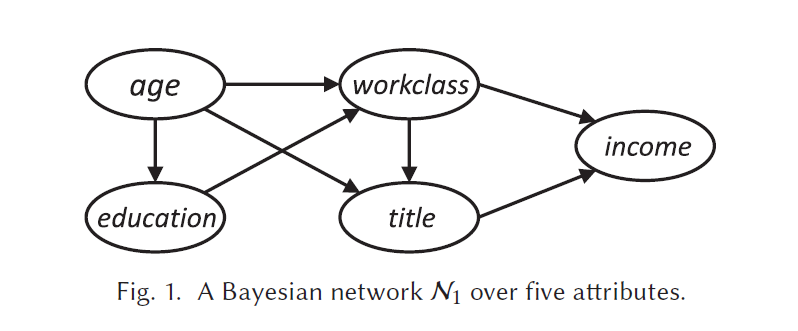
\includegraphics[scale=.35]{../graphs/figure_1.PNG}
\end{figure}
}


\frame{\frametitle{SD2011 - pMSE by number of parents}
\begin{figure}
    \caption{Model fit does not improve after $k=2$}
    \vskip -2mm
    \resizebox{.65\textwidth}{!}{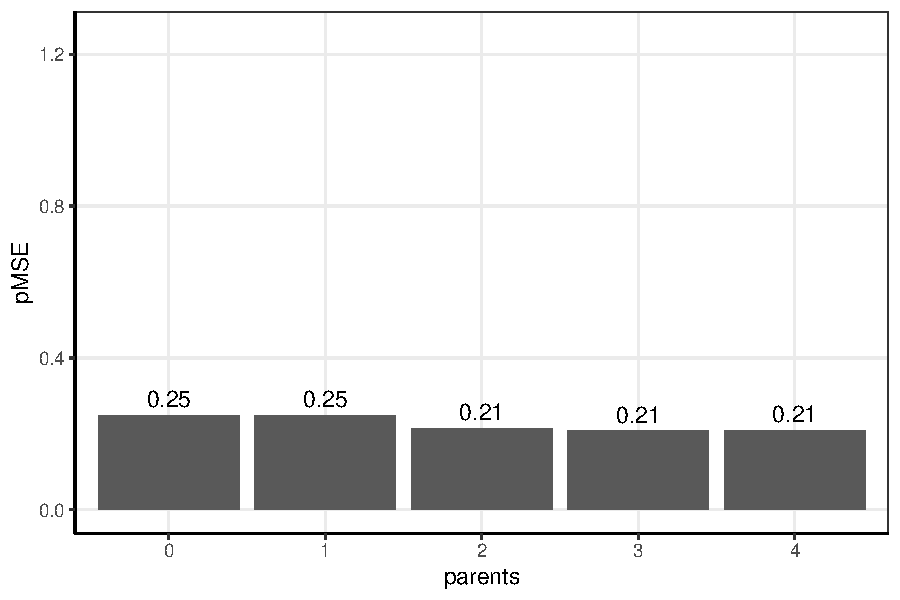
\includegraphics{../graphs/datasynthesizer/datasynthesizer_fidelity_optimize_dataset_parents.pdf}}
    \label{fig:datasynthesizer_fidelity_optimize_dataset_parents}
\end{figure}
}

\frame{\frametitle{Two-way utility: pMSE for pairs of variables}
\begin{figure}
    \caption{SD2011(a) -- Raw data}
    \vskip -2mm
    \resizebox{.7\textwidth}{!}{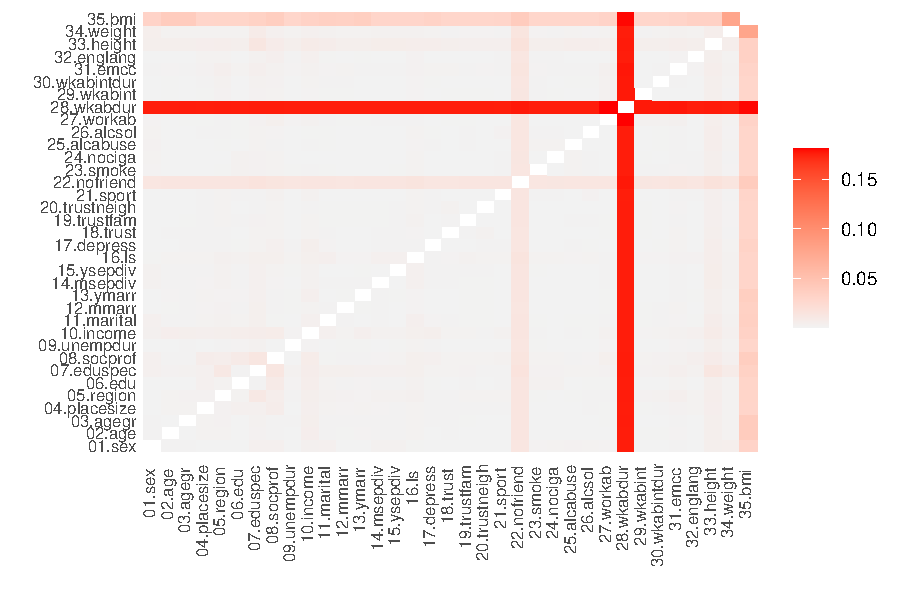
\includegraphics{../graphs/datasynthesizer/datasynthesizer_fidelity_twoway_sd2011_presentation.pdf}}
    \label{fig:ds_fidelity_two_way_subfig-a}
\end{figure}
}

\frame{\frametitle{variable: wkabdur (Work abroad duration)}
\begin{figure}
    \caption{Captures values $<$ 0 as continuous, not missing/categorical}
    \vskip -2mm
    \resizebox{\textwidth}{!}{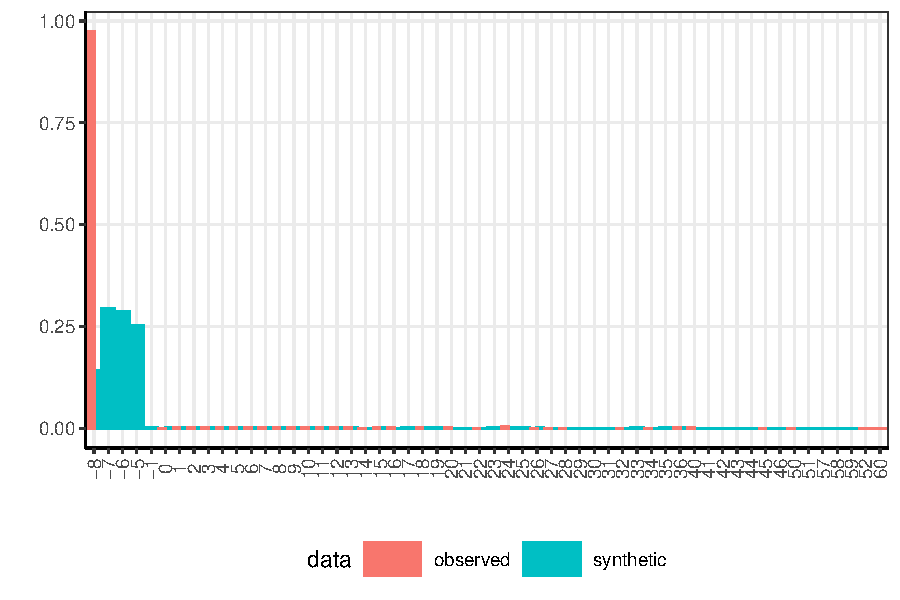
\includegraphics{../graphs/datasynthesizer/datasynthesizer_wkabdur.pdf}}
    \label{fig:ds_variable_wkabdur}
\end{figure}
}

\frame{\frametitle{Two-way utility: pMSE for pairs of variables}
\begin{figure}
    \caption{SD2011(b) -- missing are numerical values $< 0$ and `` '' categorical values}
    \vskip -2mm
    \resizebox{.70\textwidth}{!}{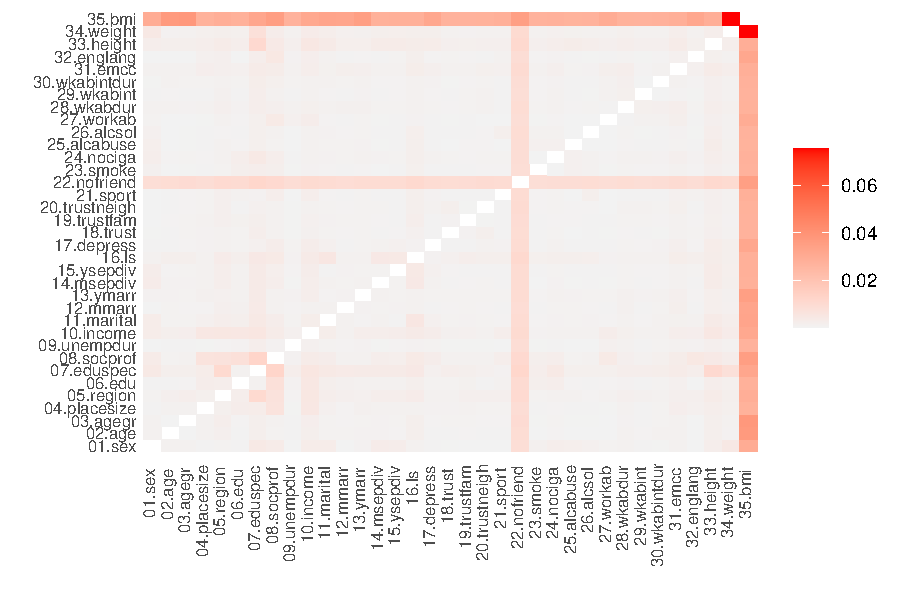
\includegraphics{../graphs/datasynthesizer/datasynthesizer_fidelity_twoway_sd2011_clean_presentation.pdf}}
    \label{fig:ds_fidelity_two_way_subfig-b}
\end{figure}
}

\frame{\frametitle{variable: bmi}
\begin{figure}
    \caption{BMI $<$ 20 is underweight/malnourished}
    \vskip -2mm
    \resizebox{\textwidth}{!}{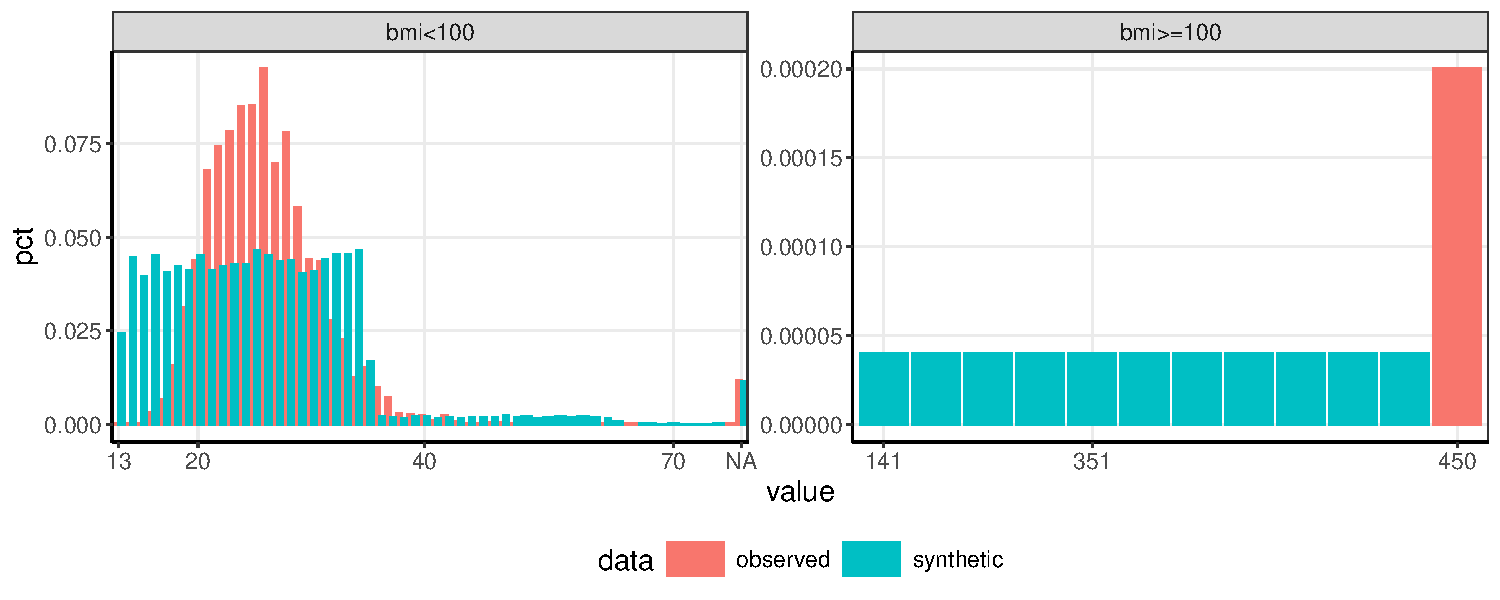
\includegraphics{../graphs/datasynthesizer/datasynthesizer_bmi.pdf}}
    \label{fig:ds_variable_bmi}
\end{figure}
}

\frame{\frametitle{Two-way utility: pMSE for pairs of variables}
\begin{figure}
    \caption{SD2011(c) -- drop generated variables (bmi and agegr)}
    \vskip -2mm
    \resizebox{.7\textwidth}{!}{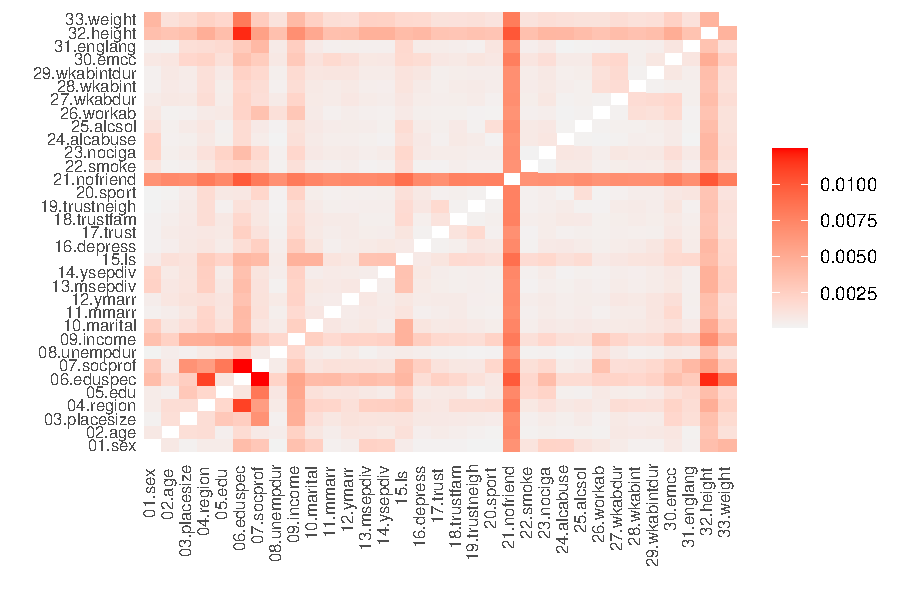
\includegraphics{../graphs/datasynthesizer/datasynthesizer_fidelity_twoway_sd2011_clean_small_presentation.pdf}}
    \label{fig:ds_fidelity_two_way_subfig-c}
\end{figure}
}

\frame{\frametitle{variable: nofriend}
\begin{figure}
    \caption{Doesn't capture rounding/discontinuity}
    \vskip -2mm
    \resizebox{\textwidth}{!}{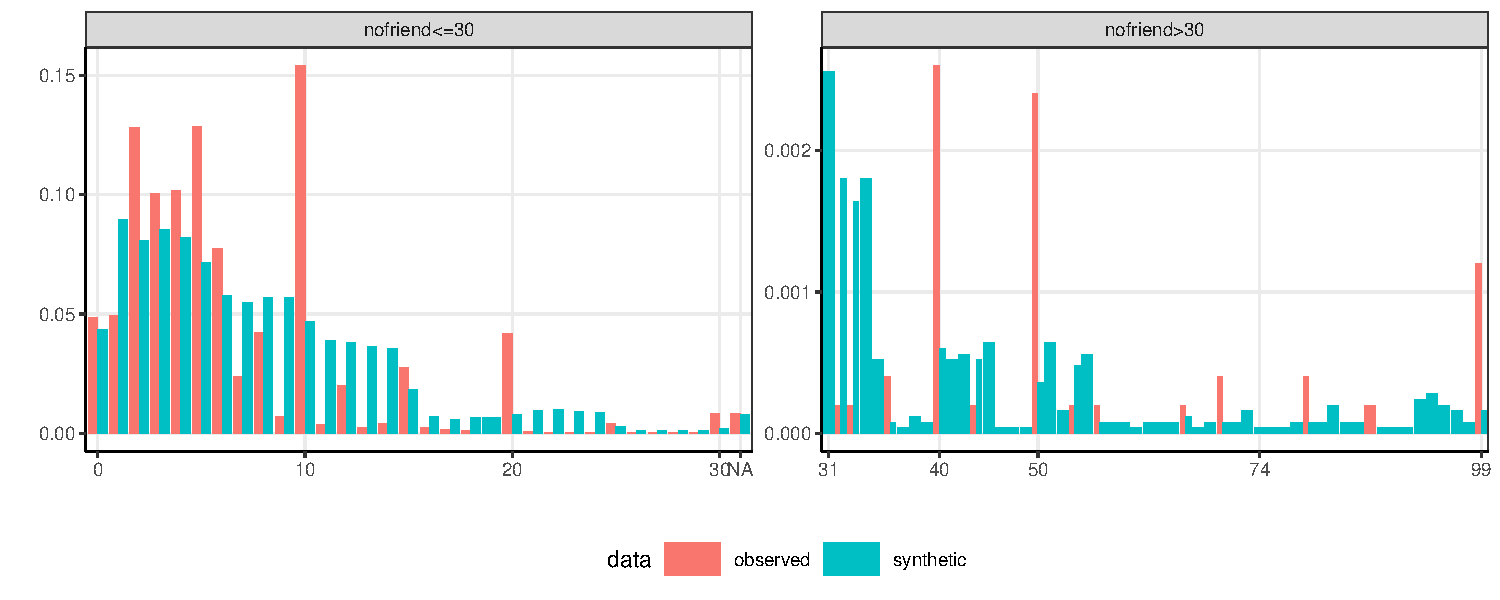
\includegraphics{../graphs/datasynthesizer/datasynthesizer_nofriend.pdf}}
    \label{fig:ds_variable_nofriend}
\end{figure}
}

\frame{\frametitle{SD2011 - pMSE}
\begin{figure}
    \caption{We use SD2011(c) - cleaned missing values, dropped generated variables, and $k=2$}
    \vskip -2mm
    \resizebox{.65\textwidth}{!}{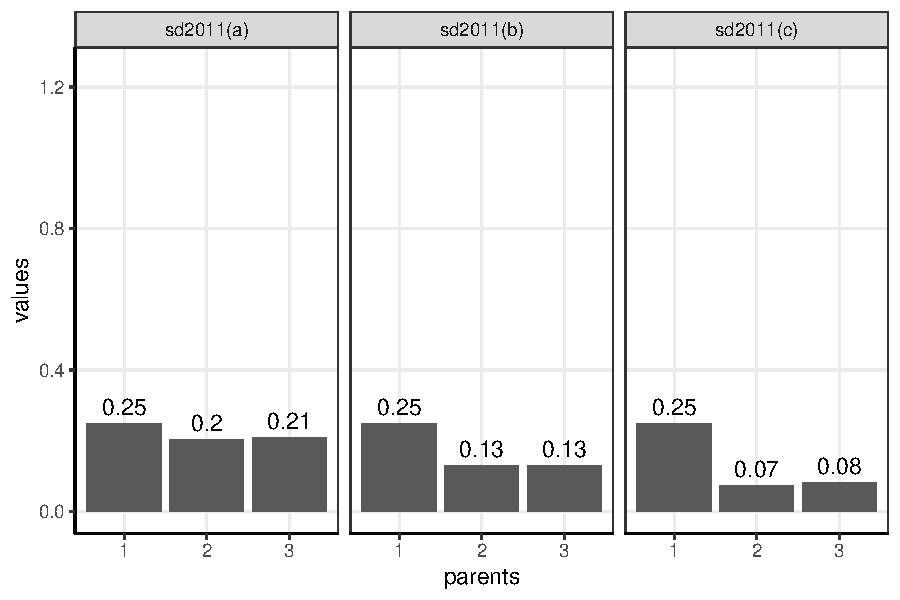
\includegraphics{../graphs/datasynthesizer/datasynthesizer_fidelity_optimize_dataset_parents_compare.pdf}}
    \label{fig:datasynthesizer_fidelity_optimize_dataset_parents_compare}
\end{figure}
}

\frame{\frametitle{Percent frequency for selected variables by parents}
\begin{figure}
    \caption{No missings if parents $<$ 2}
    \vskip -2mm
    \resizebox{\textwidth}{!}{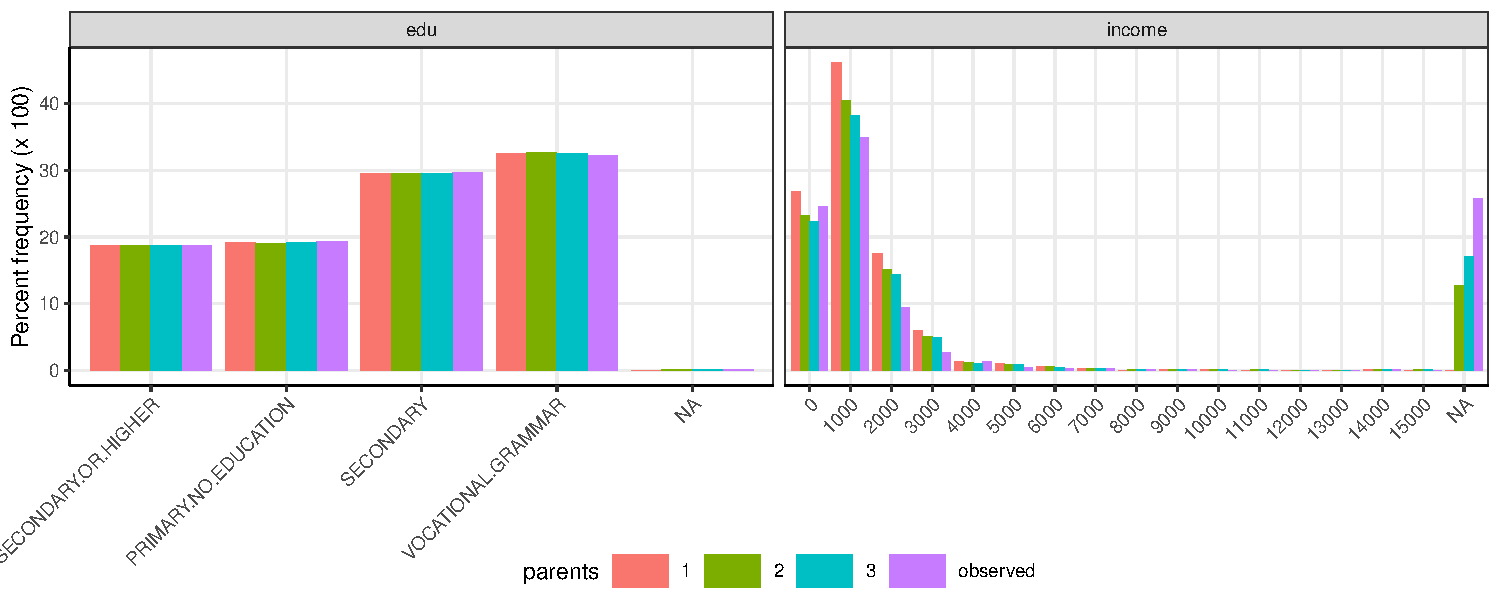
\includegraphics{../graphs/datasynthesizer/datasynthesizer_frequency_optimize_variables_parents.pdf}}
    \label{subfig:tuning_ds_variables_within_synthetic}
\end{figure}
}

\frame{\frametitle{Summary}
\begin{itemize}
    \item General lessons
    \begin{itemize}
        \item You have to `know' your data (missings, negative values, etc.)
        \item No need to replicate generated variables
    \end{itemize}
    \item DataSynthesizer lessons for SD2011
    \begin{itemize}
        \item Will only capture missing values if parents ($k$) $>=2$
        \item Better at capturing distribution of categorical variables than continuous variables
    \end{itemize}
    \item Its the only SDG that incorporates $\epsilon$ DP as a setable hyperparameter
\end{itemize}
}


\subsection{CTGAN}\label{sec:sdg_ctgan}
\frame{\frametitle{}
Section \ref{sec:sdg}\ref{sec:sdg_ctgan}: Know your generator (CTGAN)

GANs (Goodfellow et al., 2014), simultaneously train two NN models: a generative model which captures the data distribution, and a discriminative model that aims to determine whether a sample is from the model distribution or the data distribution. 

The generative model starts off with noise as inputs and relies on feedback from the discriminative model to generate a data sample.  This goes back and forth until the discriminator cannot distinguish between the actual data and the generated data.

Unlike DataSynthesizer, GANs were created to deal with continuous variables.

}

\frame{\frametitle{Tuning CTGAN: `Primary' hyperparameters}
\begin{itemize}
    \item epochs = Number of times to train the GAN. Each new epoch can improve the model (default is 300).
    \item batch size = Number of samples to process in each step (default is 500)
\end{itemize}
\begin{table}[!h]
    \rowcolors{1}{white}{lightgray}
    \caption{Batch size and epochs = actual steps}
    \centering
    \begin{tabular}{cllll}
    \toprule
    N & Batch size & Steps per Epoch & Epochs & Actual Steps \\
    \midrule
    5.000 & 500 & 10 & 100 & 1,000 \\
    5.000 & 500 & 10 & 300 & 3,000 \\
    5.000 & 500 & 10 & 600 & 6,000 \\
    5.000 & 500 & 10 & 900 & 9,000 \\ \hline
    5.000 & 100 & 50 & 60 & 3,000 \\
    5.000 & 250 & 20 & 150 & 3,000 \\
    5.000 & 500 & 10 & 300 & 3,000 \\
    5.000 & 1.000 & 5 & 600 & 3,000 \\ 
    \bottomrule
    \end{tabular}
\end{table}
}


\frame{\frametitle{Tuning CTGAN: `Advanced' hyperparameters}
\begin{itemize}
    \item dimensionality - The number of layers in the generator/discriminator networks
    \begin{itemize}
        \item 2 hyperparameters, but same value for each
        \item discriminator\_dim (tuple or list of ints): Size of the output samples for each one of the Discriminator Layers. A Linear Layer will be created for each one of the values provided. Defaults to (256, 256).
        \item generator\_dim (tuple or list of ints): Size of the output samples for each one of the Residuals. A Residual Layer will be created for each one of the values provided. Defaults to (256, 256).  
        \end{itemize}
    \item embedding\_dim (int): Size of the random sample passed to the Generator. Defaults to 128.
    \begin{itemize}
        \item The embedding dimension essentially influences how much the information in the original data set is compressed
    \end{itemize}
\end{itemize}
}

% \section{Results}\label{sec:results}
\frame{\frametitle{CTGAN: Effect of batch size (constant steps)}
\begin{figure}
    \resizebox{.75\textwidth}{!}{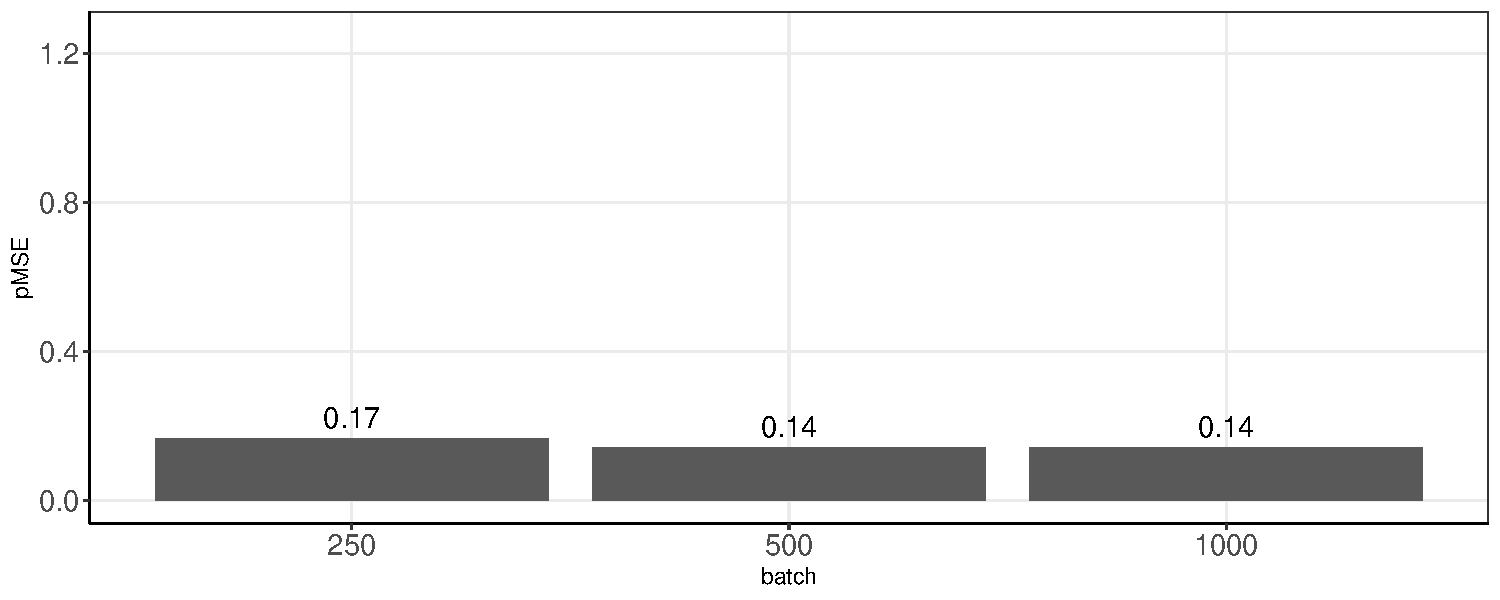
\includegraphics{../../ctgan/graphs/ctgan/ctgan_fidelity_optimize_batch_size.pdf}}
    \label{ctgan_fidelity_optimize_batch_size}
\end{figure}
}

\frame{\frametitle{CTGAN: Effect of epochs (constant batch size)}
\begin{figure}
    \resizebox{.75\textwidth}{!}{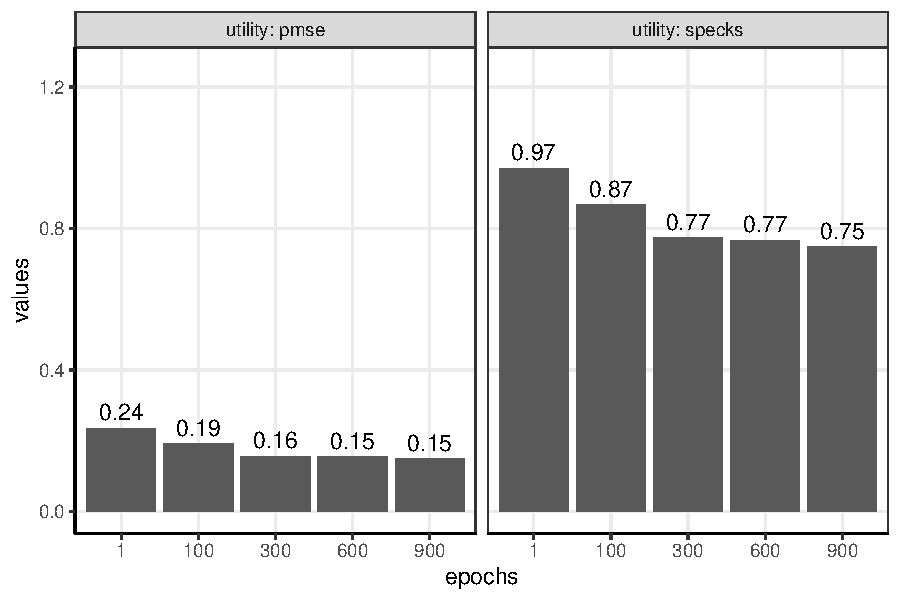
\includegraphics{../../ctgan/graphs/ctgan/ctgan_fidelity_optimize_epochs.pdf}}
    \label{ctgan_fidelity_optimize_epochs}
\end{figure}
}

\frame{\frametitle{CTGAN: Effect of dimensions}
\begin{figure}
    \resizebox{.7\textwidth}{!}{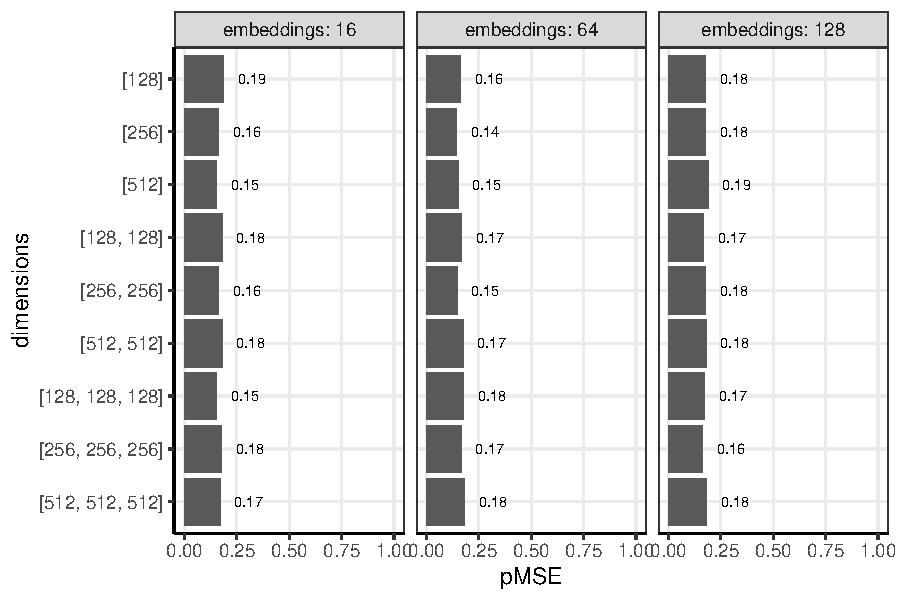
\includegraphics{../../ctgan/graphs/ctgan/ctgan_fidelity_optimize_dimensions.pdf}}
    \label{ctgan_fidelity_optimize_dimensions}
\end{figure}
}

\frame{\frametitle{variable: nofriend}
\begin{figure}
    \caption{CTGAN is better than DataSynthesizer below 30, but both are bad above 30}
    \vskip -2mm
    % \resizebox{\textwidth}{!}{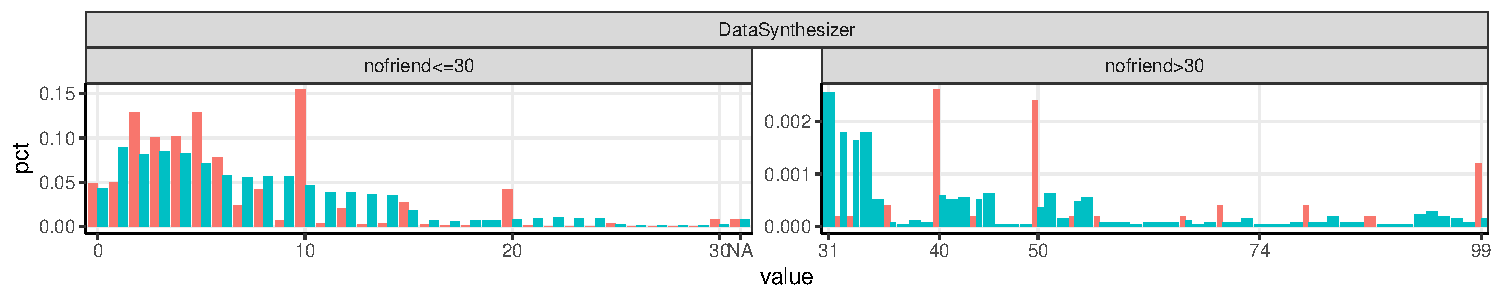
\includegraphics{../graphs/datasynthesizer/datasynthesizer_nofriend_1.pdf}}
    % \resizebox{\textwidth}{!}{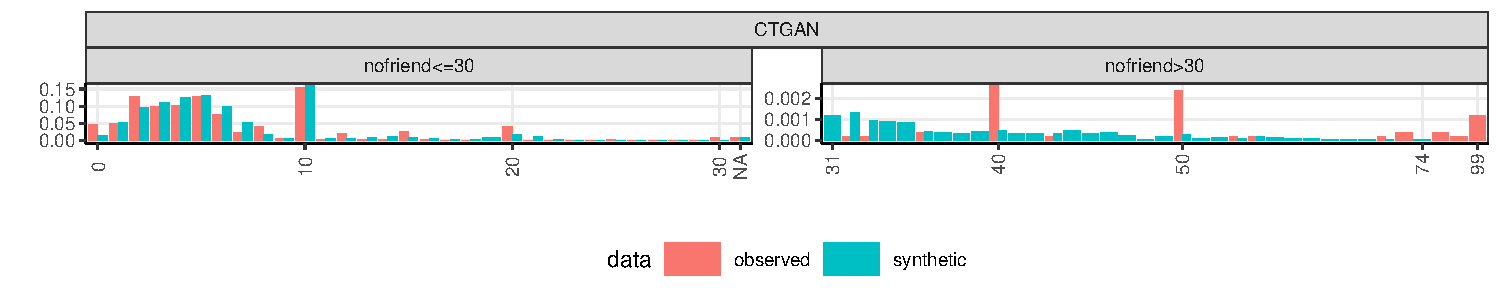
\includegraphics{../graphs/ctgan/ctgan_nofriend_1.pdf}}
    \resizebox{\textwidth}{!}{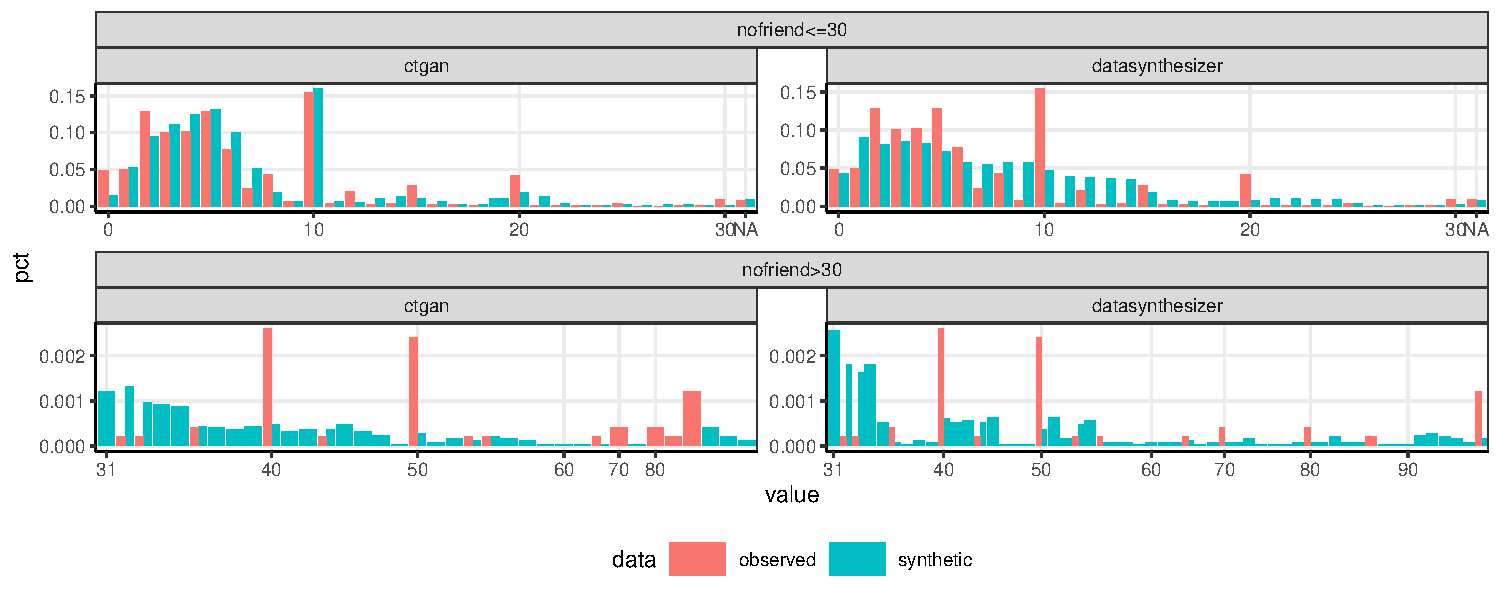
\includegraphics{../graphs/compare_ds_ctgan_nofriend_1.pdf}}
    \label{fig:ctgan_variable_nofriend}
\end{figure}
}

\frame{\frametitle{variable: bmi}
\begin{figure}
    \caption{CTGAN/DataSynthesizer estimate the median, but CTGAN is skewed a bit more to the right}
    \vskip -2mm
    \resizebox{\textwidth}{!}{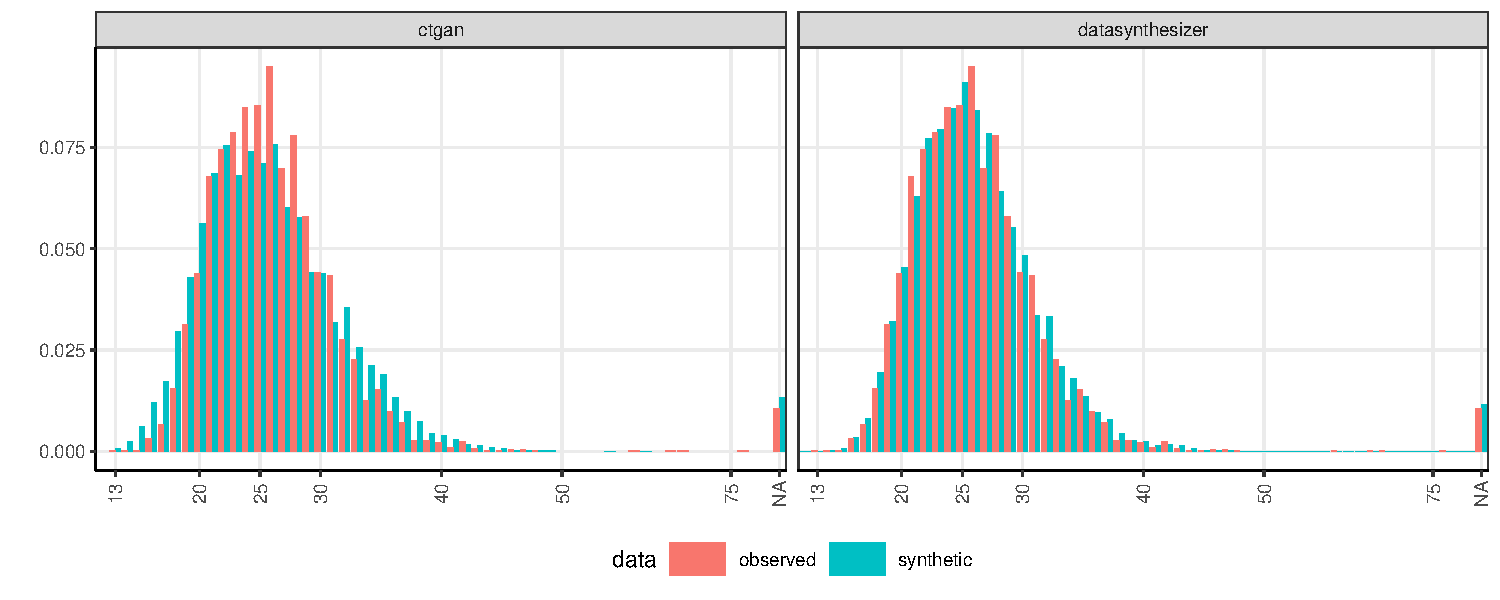
\includegraphics{../graphs/compare_ds_ctgan_bmi_1.pdf}}
    \label{fig:ctgan_variable_bmi}
\end{figure}
}


\frame{\frametitle{variable: wkabdur (Work abroad duration)}
\begin{figure}
    \caption{CTGAN does not correctly estimate the distribution, DataSynthesizer gets the median (10), but not the rounding}
    \vskip -2mm
    \resizebox{\textwidth}{!}{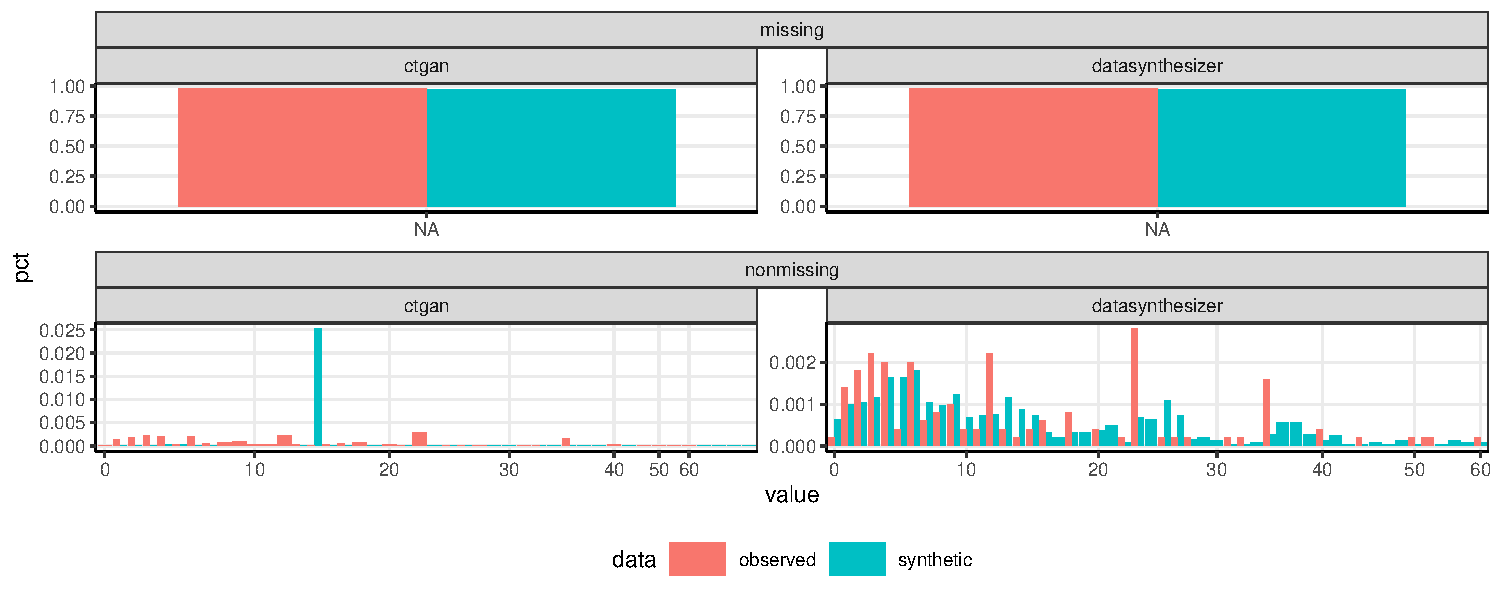
\includegraphics{../graphs/compare_ds_ctgan_wkabdur_1.pdf}}
    \label{fig:ctgan_variable_wkabdur}
\end{figure}
}

\frame{\frametitle{Summary}
\begin{itemize}
    \item CTGAN is not a good SDG
    \item But, CTGAN is not the only GAN
    \item Distinguish between the package and the synthesizer
    \item Can we make a better GAN?  Yes, we can \dots
\end{itemize}
}

\subsection{Synthpop}\label{sec:sdg_synthpop}
\frame{\frametitle{}
Section \ref{sec:sdg}\ref{sec:sdg_synthpop}: Know your generator (Synthpop)

Synthpop, R package, uses methods based on classification and regression trees (CART, developed by Breiman et al. (1984)), which can handle mixed data types and is non-parametric. Synthpop synthesises the data sequentially, one variable at a time; the first is sampled, then the following are predicted using CART (in the default mode) with the previous variables used as predictors. This means that the order of variables is important (and can be set by the user). 
}

\frame{\frametitle{SD2011 - pMSE}
\begin{figure}
    \caption{}
    \vskip -2mm
    \resizebox{.7\textwidth}{!}{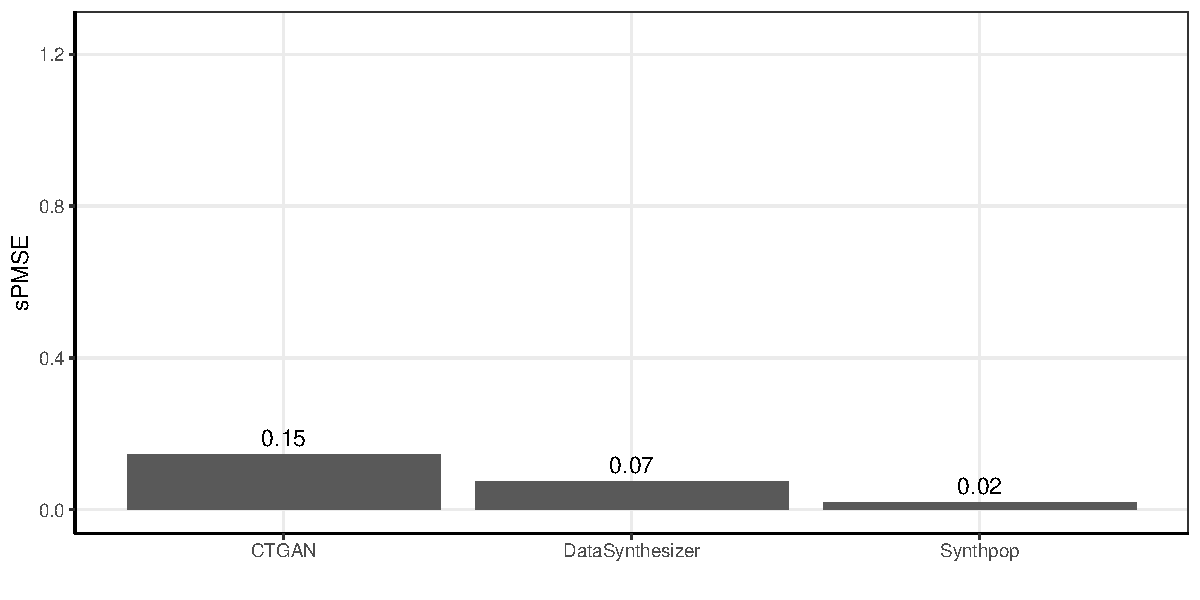
\includegraphics{../graphs/graph_fidelity_compare_dataset.pdf}}
    \label{fig:graph_fidelity_compare_dataset}
\end{figure}
}

\frame{\frametitle{Two-way utility: pMSE for pairs of variables}
\begin{figure}
    \caption{}
    \vskip -2mm
    \resizebox{\textwidth}{!}{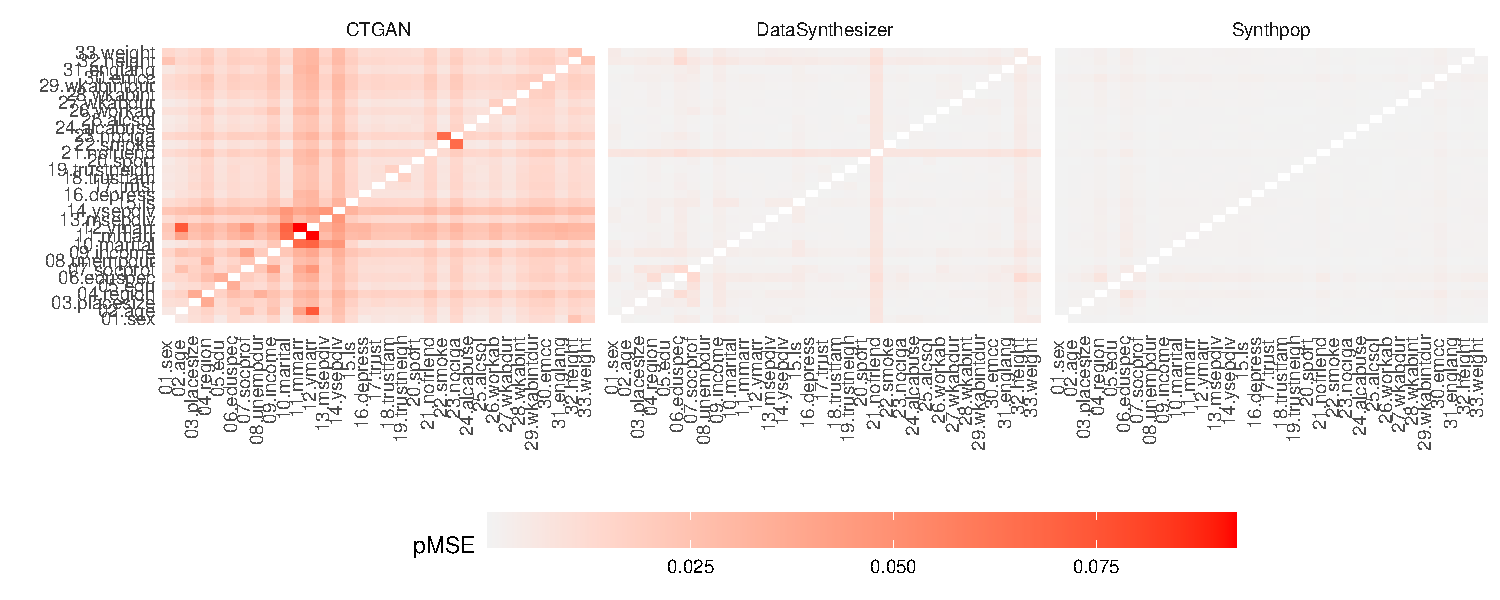
\includegraphics{../graphs/graph_fidelity_twoway_compare.pdf}}
    \label{fig:graph_fidelity_twoway_compare}
\end{figure}
}

\frame{\frametitle{variable: nofriend}
\begin{figure}
    \caption{Synthpop captures the distribution}
    \vskip -2mm
    % \resizebox{\textwidth}{!}{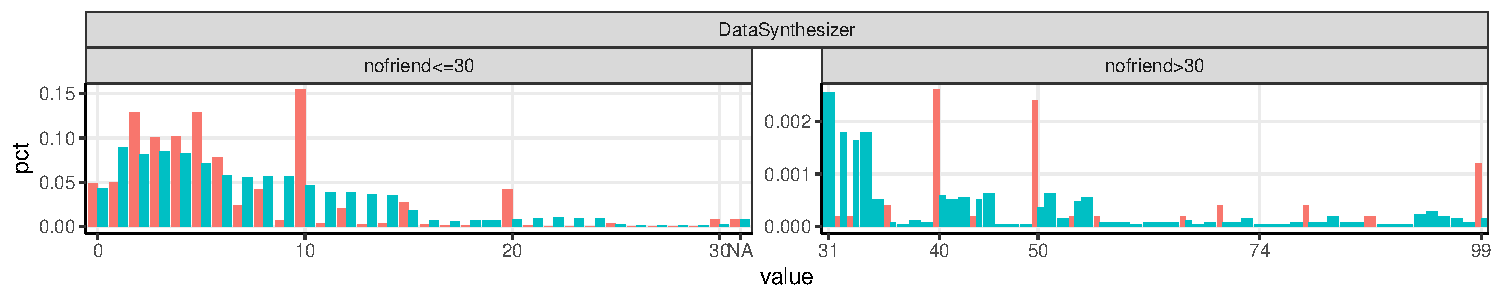
\includegraphics{../graphs/datasynthesizer/datasynthesizer_nofriend_1.pdf}}
    % \resizebox{\textwidth}{!}{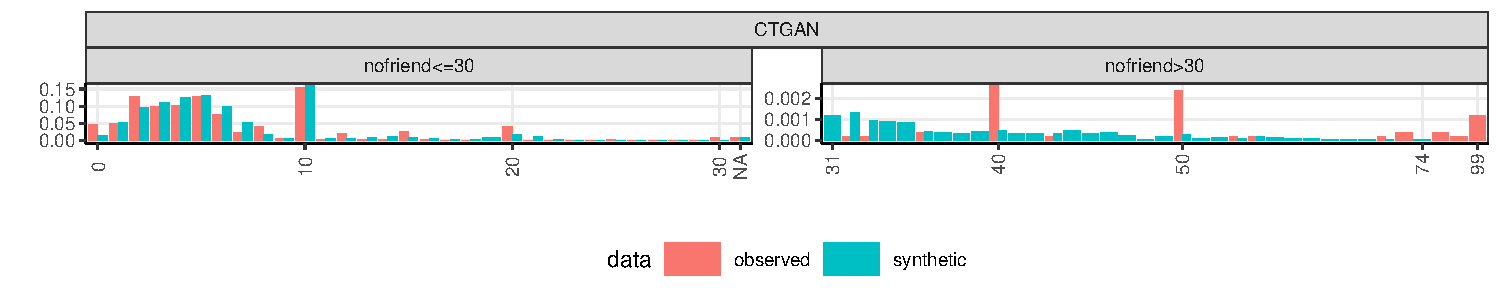
\includegraphics{../graphs/ctgan/ctgan_nofriend_1.pdf}}
    \resizebox{\textwidth}{!}{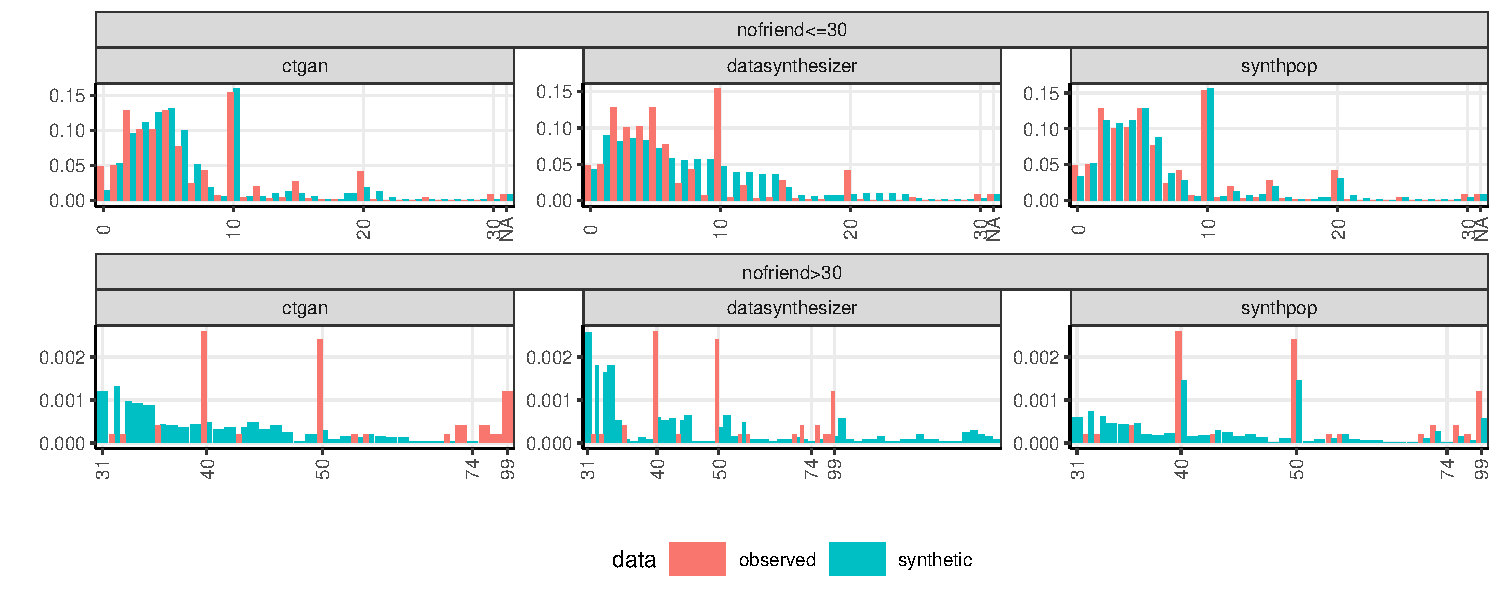
\includegraphics{../graphs/compare_nofriend_1.pdf}}
\end{figure}
}

\frame{\frametitle{variable: bmi}
\begin{figure}
    \caption{DataSynthesizer is similar to Synthpop}
    \vskip -2mm
    \resizebox{\textwidth}{!}{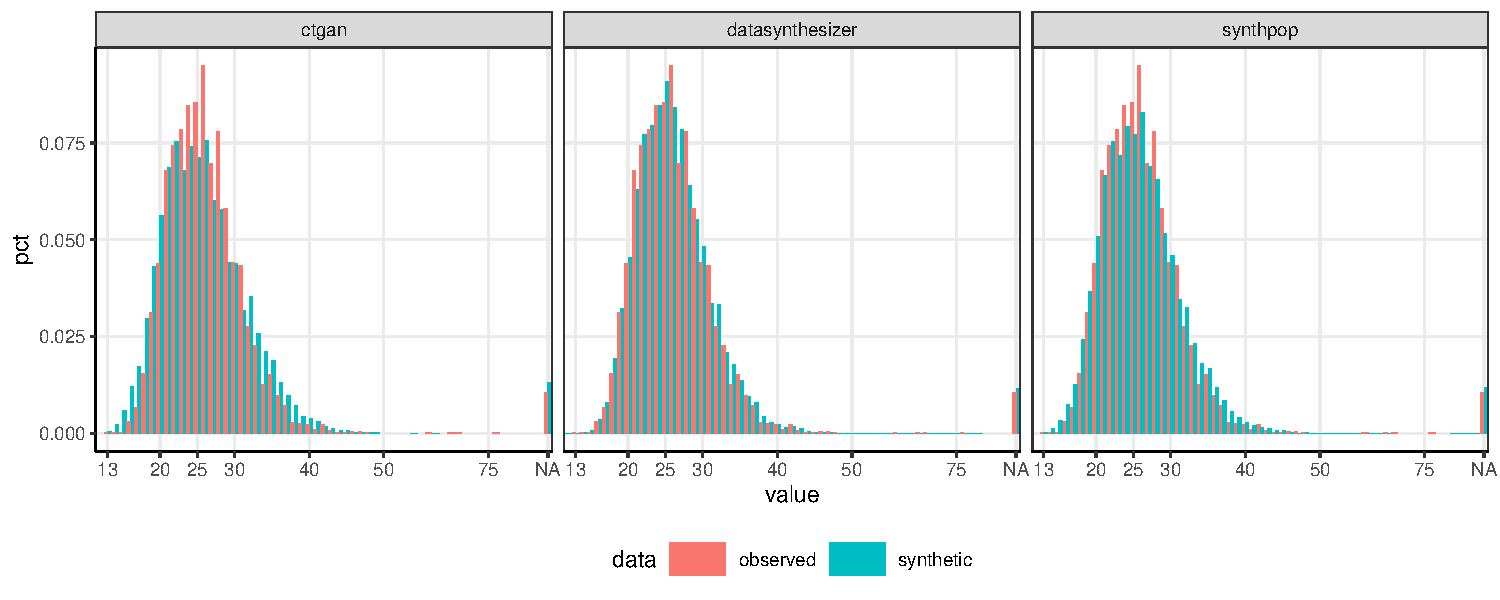
\includegraphics{../graphs/compare_bmi_1.pdf}}
\end{figure}
}


\frame{\frametitle{variable: wkabdur (Work abroad duration)}
\begin{figure}
    \caption{Like CTGAN, Synthpop is higher than median (10), but is better with the distribution than CTGAN}
    \vskip -2mm
    \resizebox{\textwidth}{!}{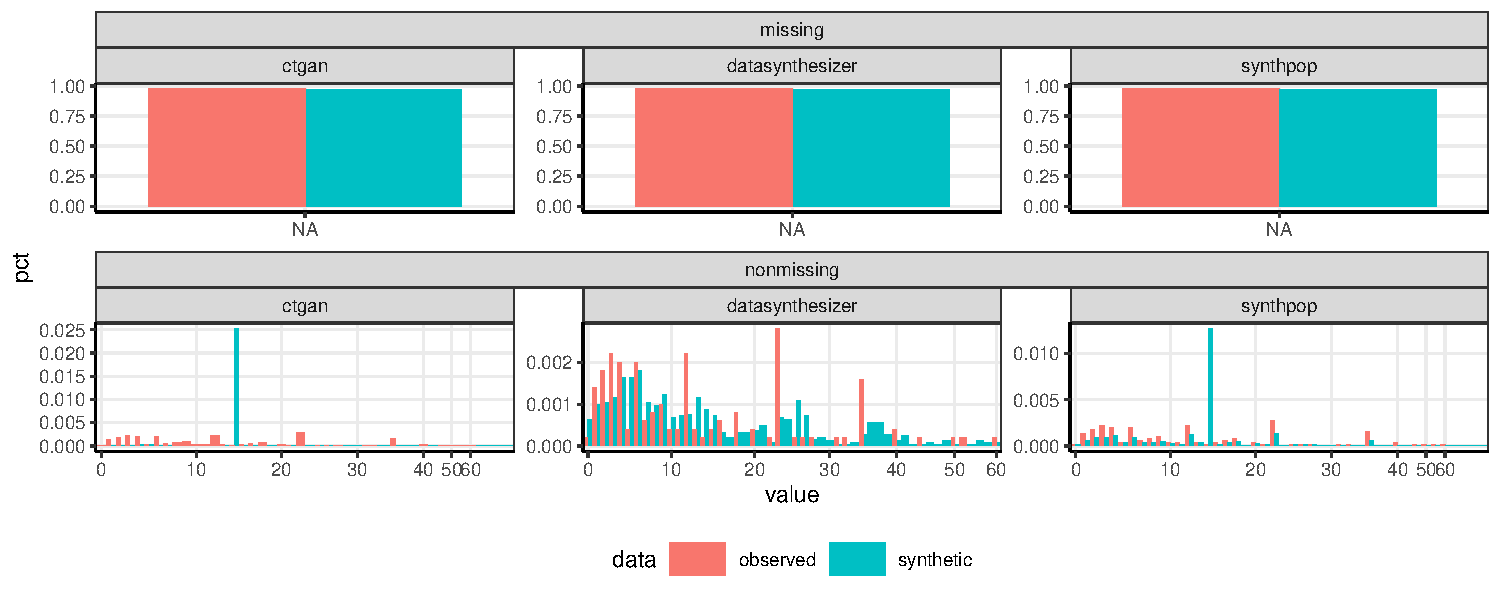
\includegraphics{../graphs/compare_wkabdur_1.pdf}}
\end{figure}
}

\frame{\frametitle{Efficiency - duration in seconds}
\vskip -5mm
\begin{table}[ht]
    \centering
    \vskip -2mm
    \rowcolors{1}{white}{lightgray}
    \resizebox{\textwidth}{!}{% latex table generated in R 4.4.0 by xtable 1.8-4 package
% Fri Jul 19 16:14:31 2024
\begin{tabular}{llrrrr}
  \toprule
version & description & ctgan & datasynthesizer & synthpop (csv) & synthpop (package) \\ 
  \midrule
v00 & Raw (SD2011) & 331.01 & 245.37 & 2132.12 & 5474.39 \\ 
  v01 & Without eduspec or wkabdur & 290.30 & 264.43 & 10.99 & 8.45 \\ 
  v02 & Without wkabdur & 337.07 & 351.76 & 13.96 & 11.02 \\ 
  v03 & Without eduspec & 306.46 & 351.24 & 11.39 & 8.92 \\ 
  v04 & Last variables: eduspec-wkabdur & 374.57 & 344.02 & 14.23 & 287.85 \\ 
  v05 & Last variables: wkabdur-eduspec & 419.60 & 339.92 & 14.60 & 3657.55 \\ 
  v06 & as.numeric(wkabdur) and last variable: eduspec & 356.02 & 347.36 & 14.12 & 11.05 \\ 
  v07\_1\_20 & + 1 factor variable (20 values) & 339.05 & 264.96 & 42.23 &  \\ 
  v07\_1\_25 & + 1 factor variable (25 values) & 400.28 & 326.84 & 137.47 &  \\ 
  v07\_1\_30 & + 1 factor variable (30 values) & 339.73 & 269.72 & 363.18 &  \\ 
  v07\_2\_20 & + 2 factor variable (20 values) & 369.74 & 339.45 & 74.96 &  \\ 
  v07\_2\_25 & + 2 factor variable (25 values) & 364.56 & 361.81 & 631.43 &  \\ 
  v07\_2\_30 & + 2 factor variable (30 values) & 373.25 & 346.15 & 1222.54 &  \\ 
  v07\_3\_20 & + 3 factor variable (20 values) & 393.99 & 369.58 & 122.77 &  \\ 
  v07\_3\_25 & + 3 factor variable (25 values) & 401.03 & 383.40 & 881.53 &  \\ 
  v07\_3\_30 & + 3 factor variable (30 values) & 394.44 & 424.64 & 3654.59 &  \\ 
   \bottomrule
\end{tabular}
}
    \label{table:table_sd2011_duration}
\end{table}
}

\frame{\frametitle{Summary}
\begin{itemize}
    \item Advantages
    \begin{itemize}
        \item Synthpop is an excellent SDG
        \item Much better than CTGAN/DataSynthesizer
    \end{itemize}
    \item Disadvantages
    \begin{itemize}
        \item Questions about privacy (not addressed here)
        \item Issues with high dimensional data
    \end{itemize}
\end{itemize}
}


\section{Conclusion}\label{sec:conclusion}
\frame[c]{\frametitle{}
\centering
Section \ref{sec:conclusion}: Conclusion
}

\frame{\frametitle{Results}
\begin{itemize}
    \item Know the data
    \begin{itemize}
        \item Cleaning/preprocessing are important
        \item 
    \end{itemize}
    \item Know your synthesizer
    \begin{itemize}
        \item Synthpop is the best SDG, but struggles with high dimensional data
        \item DataSynthesizer is the only one to offer a hyperparameter for privacy
        \item CTGAN is bad, but maybe there is a better GAN
    \end{itemize}
\end{itemize}
}


\end{spacing}
\end{document}

